\chapter{Background}

In this chapter we will go through the fundamental mathematics and concepts behind the \textit{Convolutional Neural Network} (CNN) model, in order to be able to recognize which operations that can be hardware-accelerated. It gives a basic introduction to both general neural networks and \textit{CNNs}. The last section gives an overview of the research and state-of-the-art hardware implementations of CNNs. 

\section{Artificial Neural Networks}

An \textit{Artificial Neural Network} (ANN) is a computational model that is used for machine learning and pattern recognition. The name and basic concept is inspired by how the animal brain uses a network of neurons to recognize and classify objects. 

An ANN can intuitively be viewed as a probabilistic classifier. Depending on the input data it will output the probability that the data belongs to a certain \textit{class} (e.g. an object in an image or an investment decision). As the brain it can be trained to recognize different classes by being provided a set of labeled training data, e.g. a set of faces and a set of non-faces. It can then learn to decide whether a image contains a face or not. This is called supervised learning. The network can also be trained unsupervised, by providing it with a set of unlabeled images. It will then learn to recognize a set of classes, but will be unable to label them.  

The topology of an ANN is a number of layers containing a set of so-called neurons. A neuron takes as in a set of inputs (e.g. image pixels), where each input is associated with a respective weight. The input and the weight are then multiplied and summed, and the result is used to calculate a non-linear activation function. More formally a neuron is defined as follows: 

\begin{equation*}
Input: \{x_1, x_2,\dots, x_n\} = \mathbf{x} 
\end{equation*}

\begin{equation*}
Output: f(\mathbf{w^{T}x)} = f(\sum_{i=1}^{n}w_i x_i + b)
\end{equation*}

\textbf{w} is the connection weights, b is the neuron bias and \textit{f(...)} is the activation function. \textit{f(...)} tends to be either:

\begin{equation*}
Sigmoid: f(z) = \frac{1}{1 - e^{-z}}, \in [0,1]
\end{equation*}

or 

\begin{equation*}
Hyperbolic tagent: f(z) = tanh(z) = \frac{e^z - e^{-z}}{e^z + e^{-z}}, \in [-1,1]
\end{equation*}

An ANN consist of $ n_l $ layers, each containing a set of neurons. The first layer is \textit{the input layer}, and the last layer is \textit{the output layer}. The layers in between are called \textit{the hidden layers}. Each layer uses the previous layer output as input. The input layer is provided with the initial input and calculates its activation functions (one for each neuron). The result is propagated to the first hidden layer, and continues up until it reaches the output layer - which provides the final output. This is known as a \textit{feedforward neural network.}

The network takes in two parameters, $ (\mathbf{W, b}) = (\mathbf{w^{(1)}, b^{(1)}}, 
\mathbf{w^{(2)}, b^{(2)}}, \dots , 
\mathbf{w^{(n_l)}, b^{(n_l)}}) $. Then $ w_{ij}^l $ denotes the weight between neuron j in layer l, and neuron i in layer l+1. $ b_i^l $ denotes the bias associated with neuron i in layer l+1.

During the training of the network it is the parameters $ (\mathbf{W, b}) $ that are altered in order to adapt the network to the training data. This is done by providing the network with a set of training examples, where we provide an input and an expected output. We then use a cost function to compute the error of the actual output. Our goal is to minimize the cost function, so the actual output is as close as possible to the expected output. This can be done by a technique called gradient decent. 

Let the cost function for a single training example $(x,y)$ be defined as follows:

\begin{equation*}
	Cost(\mathbf{w},b; x, y) = \frac{1}{2}(h_{\mathbf{w},b}(x) - y)^2
\end{equation*}

Where $ x $ is the input, $ h_{\mathbf{w},b}(x) $ is the actual output of the ANN and \textit{y} is the correct output.
Then the cost function for \textit{m} training examples $ ((x^{1}, y^{1}), (x^{2}, y^{2}), \dots, (x^{m}, y^{m})) $ is:

\begin{equation*}
	Cost(\mathbf{w},b) = \frac{1}{m}\sum_{i=1}^{m}Cost(\mathbf{w},b;x^{(i)},y^{(i)}) + \frac{\lambda}{2}
	\sum_{l=1}^{n_l-1}\sum_{i=1}^{s_l}\sum_{j=1}^{s_l+1}
	(\mathbf{w}_{ji}^{l})^2
\end{equation*}
 
The first term is simply the average sum-of-squares error term. The second term is the \textit{text}regularization term, or \textit{weight decay term}, which tends to reduce \textit{overfitting}.

Based on this we can use \textit{gradient decent} to compute how we should alter the weights in order to reduce the cost function. One iteration of gradient descent updates \textbf{w} and \textit{b} as follows:

\begin{equation*}
	\mathbf{w}_{ij}^{(l)} = \mathbf{w}_{ij}^{(l)} - \alpha\frac{\partial}{\partial\mathbf{w}_{ij}^{(l)} }Cost(\mathbf{w},b)
\end{equation*}

\begin{equation*}
	\mathbf{b}_{i}^{(l)} = \mathbf{b}_{i}^{(l)} - \alpha\frac{\partial}{\partial\mathbf{b}_{i}^{(l)} }Cost(\mathbf{w},b)
\end{equation*}

Where $ \alpha $ is the learning rate, which is a predetermined constant. Note that this would only make us able to compute the gradient for the output layer. In order to perform gradient decent on the hidden layers, we need to propagate the error from the output layer backwards, to the hidden layers. For this we use the \textit{backpropagation algorithm}. Let $ o_i^{(l)} $ denote the output of the $i$th neuron in layer $l$, and $z_k^{(l)}$ is the weighted sum of the inputs plus the bias for the $k$th neuron in layer l. Then the \textit{backpropagation algorithm} can be formalized as follows: 

\begin{enumerate}
	\item Perform a feedforward pass, computing the output of every layer.
	\item For each output neuron k in the output layer, compute: 
	\begin{equation*}
		\delta_k = \frac{\partial}{\partial z_{k}^{(n_l)} }Cost(\mathbf{w},b; x, y) = -o_k^{n_l}(1-o_k^{n_l})(y_k-o_k^{n_l})
	\end{equation*} 
	\item For each hidden layer $ l = n_l - 1, n_l - 2,\dots, 2 $ compute: 
	\begin{equation*}
		\delta_i^{l} = o_i^l(1-o_i^l)\sum_{j=1}^{s_{l+1}} w_{ij}^l \delta_j^{l+1} 
	\end{equation*}
	\item Compute the partial derivative for each weight and bias:
	\begin{equation*}
		\frac{\partial}{\partial\mathbf{w}_{ij}^{(l)} }Cost(\mathbf{w},b; x, y) = o_j^{(l)}\delta_i^{(l+1)}
	\end{equation*}
	
	\begin{equation*}
		\frac{\partial}{\partial\mathbf{b}_{i}^{(l)} }Cost(\mathbf{w},b; x, y) = \delta_i^{(l+1)}
	\end{equation*}
\end{enumerate}
	
Now, combining \textit{gradient decent} and the \textit{backpropagation algorithm} we can describe an algorithm to train our network: 

\begin{enumerate}
	\item Initialize the weights $ \mathbf{w}^{(l)} $ and $ b^{l} $ for all \textit{l}.
	\item Do steps 3 to 5 until the $ Cost(\mathbf{w}, b; x, y) $ function is low enough or converges. This is referred to as an \textit{epoch}. 
	\item Set $ \Delta\mathbf{w}^{(l)} := 0 $ and $ \Delta b^{(l)} := 0 $ for all \textit{l}.
	\item For i = 1 to m,
		\begin{enumerate}
			\item Use the backpropagation algorithm to compute $ \nabla_\mathbf{w^{(l)}}Cost(\mathbf{w}, b;x,y) $ and $ \nabla_b^{(l)}Cost(\mathbf{w}, b;x,y) $.
			\item  Set $ \Delta\mathbf{w}^{(l)} := \Delta\mathbf{w}^{(l)} + \nabla_\mathbf{w^{(l)}}Cost(\mathbf{w}, b;x,y) $. 
			\item  Set $ \Delta b^{(l)} := \Delta b^{(l)} + \nabla_{b^{(l)}}Cost(\mathbf{w}, b;x,y) $. 
		\end{enumerate}
	\item Update the parameters:
		\begin{equation*}
			\mathbf{w}^{(l)} = \mathbf{w}^{(l)} - \alpha[(\frac{1}{m}\Delta\mathbf{w}^{(l)}) + \lambda\mathbf{w}^{(l)}]
		\end{equation*}
		
		\begin{equation*}
			b^{(l)} = b^{(l)} - \alpha[\frac{1}{m}\Delta b^{(l)}]
		\end{equation*}
\end{enumerate}



\section{Convolutional Neural Network}

\textit{Convolutional Neural Network}\cite{LeCun1998} (CNN) is a variation of the \textit{Artificial Neural Network} model, which is mainly used for object recognition in images. It addresses three major problems the standard ANN model faces when it comes to object recognition. First, even small images contains a large amount of pixels/inputs, e.g. a $ 32 \times 32 $ image contains 1024 pixels/inputs. A fully connected network with 100 hidden units would then end up with $ 1024 \times 100 $ weights that needs to be calculated in the first layer! Making it computationally infeasible and not scalable. Second, objects of the same class are seldom exactly alike, something the network has to take into consideration. While possible, the network would have to be very large, would probably contain several neurons with similar weight vectors positioned at different places in the network, and would require a very large number of training samples. Third, a fully connected ANN does not take into consideration the topology of the input. An image has a strong 2D spatial locality correlation, which makes it possible to combine low-order features (edges, end-points etc.) into higher-order features.  


\begin{figure}[h!]
  \centering
      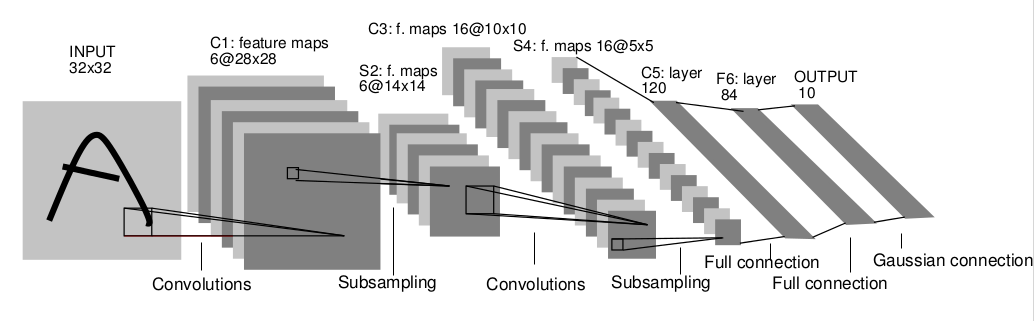
\includegraphics[width=1.0\textwidth]{Figures/Background/convnet}
  \caption{An example CNN, the LeNet-5\cite{LeCun1998}. }
\end{figure}

The CNN model adds two additional types of layers, in addition to the standard ANN layers: a convolution layer and a pooling/subsampling layer.

The idea behind the two new layers is to exploit the strong 2D local structure of images, i.e. pixels close to each other are highly correlated. By using local correlation one can extract and combine small local features (e.g. edges, corners, points) into higher-order features (e.g. nose, mouths, forehead), which can in the end be recognized as an object (e.g. a face). 

Intuitively, the convolution layer performs the feature extraction by applying a filter (kernel) on the whole image, and puts the result in a corresponding feature map. E.g. if the filter extracts vertical edges, only the vertical edges from the original image would remain in the resulting feature map. Thus you can extract different features by having several feature maps with different filters.  

Formally we can define a 2D convolution as follows. Let $ x_{ij} $ denote a value of the input matrix, $ w_{mn} $ denotes a value in a $ k \times k $ kernel matrix, and $ o_{ij} $ denotes a value of the output matrix. Then we get the following formula:

\begin{equation*}
o_{ij} = \sum_{m=1}^{k}\sum_{n=1}^{k} x_{i+m, j+n}w_{mn}
\end{equation*}


Once you have detected a feature, the exact position become less important. For example, the distance between the mouth and the eyes tend to vary between persons. So in order to make the \textit{CNN} not too sensitive to the relative placement of features, the accuracy of the feature map needs to be reduced. This can be done by partitioning the feature map into equal sized non-overlapping matrices, and then perform a pooling operation on each respective matrix. There are two types of pooling operations which are used for CNNs: 

\begin{itemize}
	\item \textit{Max-pooling} extracts the maximum value of the matrix.
	\item \textit{Average-pooling} extracts the average value of all the elements in the matrix.
\end{itemize}

In our solution we have opted for the max-pooling model, since its implementation is both easier and requires less resources. Formally it can be defined as:

\begin{equation*}
o_{ij} = max(x_{})
\end{equation*}

\begin{figure}[h!]
  \centering
      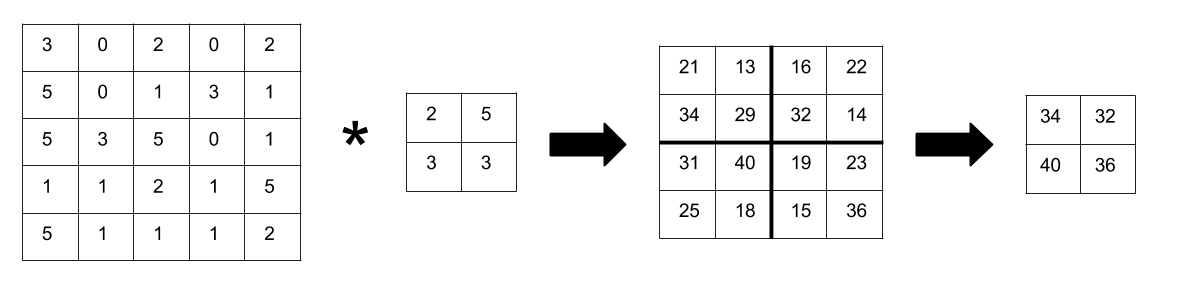
\includegraphics[width=1.0\textwidth]{Figures/Background/Convolution-Maxpooling}
  \caption{Illustration of the convolution and subsampling/max-pool layers. First the input image is convolved with the kernel, then the resulting feature map is subsampled/max-pooled.}
\end{figure}

\section{Related Work}
The mathematical fundamentals for Convolutional Neural Networks was introduced as early as in the 1980s by Kunihiko Fukushima\cite{Fukushima1980}\cite{Fukushima1982}, in form of the \textit{neocognitron} model. The model was later improved in 1998 by  Yann LeCun, Léon Bottou, Yoshua Bengio, and Patrick Haffner - who introduced the \textit{Convolutional Neural Network} model. In 2003 the model was simplified by Patrice Simard, David Steinkraus, and John C. Platt \cite{Simard2000}, in an attempt to make it easier to implement. The paper also mentions two of the main issues with CNNs, size of the training set and time spent training. In order to achieve high enough accuracy a CNN requires thousands of training samples, which needs to be labeled. Processing all of these samples and fine-tuning the networks takes a great amount of processing power, causing training to take days or weeks. These issues are the ones that caused CNNs not to gain popularity before mid-2000. The rise of the Internet, digital cameras, and Big Data have provided us with vast amounts of images which can be used for training, and improvement in the speed and sophistication of computer hardware have reduced the training time from days/weeks to hours. E.g. \cite{Cires2003} purposes a GPU implementations which reduced the epoch training time from 35 hours to 35 minutes. 

These recent advancements have renewed the interest in neural networks, and increased the research done on the field. As a result CNNs have become a leading model within pattern recognition for computer vision. This can be illustrated by the fact that CNNs implementations have won several pattern recognition contests in the period 2009-2012, including IJCNN 2011 Traffic Sign Recognition Competition\cite{Ciresan2012} and the ISBI 2012 Segmentation of Neuronal Structures in Electron Microscopy Stacks challenge\cite{DanC.Ciresan2012}.


In \cite{Farabet2009} a CNN was implemented on a Virtex-4 SX35 FPGA from Xilinx. In this implementation all the fundamental computations was hard-wired, and controlled by a 32bit soft processor using macro-instructions. Training was done offline, and a representation of the network was provided to the soft processor. With this implementation they were able to process a $ 512 \times 384 $ grayscale image in 100\textit{ms}, i.e. 10 frames per second. 








